Dans tout le corrigé, les d{\'e}nominateurs des fractions seront toujours des entiers naturels strictement positifs.
\subsection*{Question pr{\'e}liminaire}
Pour montrer que le m{\'e}dian de deux nombres rationnels est entre ces deux nombres, calculons les diff{\'e}rences:
\begin{displaymath}
\frac{p+p^{\prime }}{q+q^{\prime }}-\frac{p}{q} =\frac{p^{\prime}q-pq^{\prime }}{(q+q^{\prime })q},\hspace{0.5cm}
\frac{p^{\prime }}{q^{\prime}}-\frac{p+p^{\prime }}{q+q^{\prime }} =\frac{p^{\prime }q-pq^{\prime }}{(q+q^{\prime })q^{\prime }}
\end{displaymath}
Elles sont strictement positives car
\begin{displaymath}
 \frac{p^{\prime }}{q^{\prime }}-\frac{p}{q}=\frac{p^{\prime }q-pq^{\prime }}{qq^{\prime }}>0
\end{displaymath}

\subsection*{Partie I.\quad M{\'e}dians et suites de Farey}
\begin{enumerate}
\item  \begin{enumerate}
 \item Les d{\'e}finitions conduisent aux tuples\footnote{suivant la terminologie du type d'objet Python} suivants 
\begin{align*}
\mathcal{M}_{2} \underbrace{\mathcal{F}_{3}}&:&  \underbrace{0}, \underbrace{\frac{1}{3}}, \underbrace{\frac{1}{2}}, \underbrace{\frac{2}{3}}, \underbrace{1} \\
\mathcal{M}_{3} \underbrace{\mathcal{F}_{4}}&:&  \underbrace{0},\underbrace{\frac{1}{4}},\underbrace{\frac{1}{3}},\frac{2}{5}, \underbrace{\frac{1}{2}}, \frac{3}{5},\underbrace{\frac{2}{3}},\underbrace{\frac{3}{4}},\underbrace{1} \\
\mathcal{M}_{4} \underbrace{\mathcal{F}_{5}}&:&  \underbrace{0},\underbrace{\frac{1}{5}}, \underbrace{\frac{1}{4}}, \frac{2}{7}, \underbrace{\frac{1}{3}}, \frac{3}{8}, \underbrace{\frac{2}{5}}, \frac{3}{7}, \underbrace{\frac{1}{2}},  \frac{4}{7}, \underbrace{\frac{3}{5}}, \frac{5}{8}, \underbrace{\frac{2}{3}}, \frac{5}{7}, \underbrace{\frac{3}{4}}, \cdots \\
\mathcal{M}_{5} \underbrace{\mathcal{F}_{6}}&:&  \underbrace{0}, \underbrace{\frac{1}{6}}, \underbrace{\frac{1}{5}}, \frac{2}{9}, \underbrace{\frac{1}{4}}, \frac{3}{11}, \frac{2}{7}, \frac{3}{10}, \underbrace{\frac{1}{3}}, \cdots
\end{align*}
\item Dans les séquences précedentes, les éléments de $\mathcal F _{i+1}$ dans $\mathcal M_i$ sont indiqués par un $\underbrace{}$.
\item On remarque que le nombre d'{\'e}l{\'e}ments de $\mathcal{M}_{2}$ est $5=2^{2}+1$. D'autre part,
\begin{align*}
\text{Nb d'élts de }\mathcal{M}_{n+1} =& \text{ Nb d'élts de }\mathcal{M}_{n}+\text{ Nb d'intervalles dans }\mathcal{M}_{n} \\
=& 2\times\text{Nb d'élts de }\mathcal{M}_{n}-1
\end{align*}
donc si, pour un certain $n$,  $\text{Card}(\mathcal{M}_{n})=2^{n}+1,$ on a aussi
\begin{displaymath}
\text{Card}(\mathcal{M}_{n+1})=2(2^{n}+1)=2^{n+1}-1 
\end{displaymath}
Ceci prouve par r{\'e}currence que 
\begin{displaymath}
 \forall n \in \N : \text{Card}(\mathcal{M}_{n})=2^{n}+1
\end{displaymath}
\end{enumerate}

\item
\begin{enumerate}
\item  Traduisons l'encadrement donn{\'e} par hypoth{\`e}se par des in{\'e}galit{\'e}s sur les num{\'e}rateurs puis exploitons le fait que ces
in{\'e}galit{\'e}s sont relatives {\`a} des nombres entiers. Il vient
\[
\left\{
\begin{array}{c}
0<p^{\prime \prime }q-q^{\prime \prime }p \\
0<p^{\prime }q^{\prime \prime }-p^{\prime \prime }q^{\prime }
\end{array}
\right. \quad \text{soit\quad }\left\{
\begin{array}{c}
1\leq p^{\prime \prime }q-q^{\prime \prime }p \\
1\leq p^{\prime }q^{\prime \prime }-p^{\prime \prime }q^{\prime }
\end{array}
\right.
\]
En multipliant la premi{\`e}re {\'e}quation par $q^{\prime }$ et la
deuxi{\`e}me par $q$, on obtient
\[
q^{\prime }+q\leq (-pq^{\prime }+p^{\prime }q)q^{\prime \prime }
\]
On en d{\'e}duit $q^{\prime \prime }\geq q+q^{\prime }$ car $p^{\prime
}q-pq^{\prime }$ est suppos{\'e} {\'e}gal {\`a} 1 dans toute la question.

\item  Consid{\'e}rons, sous les hypoth{\`e}ses de la question, $p^{\prime
\prime }$ et $q^{\prime \prime }$ tels que
\[
\frac{p^{\prime \prime }}{q^{\prime \prime }}\in \left] \frac{p}{q},\frac{%
p^{\prime }}{q^{\prime }}\right[ \cap \mathcal{F}_{n+1}
\]

Exploitons d'abord le fait que $\left] \frac{p}{q},\frac{p^{\prime }}{%
q^{\prime }}\right[ \cap \mathcal{F}_{n}=\emptyset $.\newline
Comme $\frac{p+p^{\prime }}{q+q^{\prime }}$ et $\frac{p^{\prime \prime }}{%
q^{\prime \prime }}$ sont dans $\left] \frac{p}{q},\frac{p^{\prime }}{%
q^{\prime }}\right[ $, il ne sont pas dans $\mathcal{F}_{n}$ donc $%
q+q^{\prime }>n$ et $q^{\prime \prime }>n$.\newline
Comme de plus $\frac{p^{\prime \prime }}{q^{\prime \prime }}\in \mathcal{F}%
_{n+1}$, on a obligatoirement $q^{\prime \prime }=n+1$.

Utilisons ensuite la question a. Elle prouve que $q^{\prime \prime }\geq q+q^{\prime }$. On en d{\'e}duit alors  que $q+q^{\prime }=q^{\prime \prime}=n+1$.

Le m{\'e}dian $\frac{p+p^{\prime }}{q+q^{\prime }}$ et le nombre $\frac{p^{\prime \prime }}{q^{\prime \prime }}=\frac{p^{\prime \prime }}{q+q^{\prime }}$ sont dans $\left] \frac{p}{q},\frac{p^{\prime }}{q^{\prime }}\right[ $. Si par exemple
\[
\frac{p}{q}<\frac{p^{\prime \prime }}{q+q^{\prime }}\leq \frac{p+p^{\prime }%
}{q+q^{\prime }}
\]
alors
\begin{eqnarray*}
\frac{p+p^{\prime }}{q+q^{\prime }}-\frac{p^{\prime \prime }}{q+q^{\prime }}
&\leq &\frac{p+p^{\prime }}{q+q^{\prime }}-\frac{p}{q} \\
\frac{p+p^{\prime }-p^{\prime \prime }}{q+q^{\prime }} &\leq &\frac{%
p^{\prime }q-pq^{\prime }}{(q+q^{\prime })q}=\frac{1}{(q+q^{\prime })q} \\
q(p+p^{\prime }-p^{\prime \prime }) &\leq &1
\end{eqnarray*}

La seule possibilit{\'e} est $p^{\prime \prime }=p+p^{\prime }$. Un calcul
analogue dans le cas o{\`u} $\frac{p^{\prime \prime }}{q^{\prime \prime }}$
est de l'autre c{\^o}t{\'e} du m{\'e}dian ach{\`e}ve de montrer que ce
m{\'e}dian est le seul {\'e}l{\'e}ment possible de $\mathcal{F}_{n+1}$ entre
$\frac{p}{q}$ et $\frac{p^{\prime }}{q^{\prime }}$.
\end{enumerate}

\item \begin{enumerate}
 \item Supposons que $x<y$ sont deux éléments consécutifs de $\mathcal F_{n+1}$ dont aucun n'est dans $\mathcal F_n$. Il existe alors ds éléments consécutifs $a<b$ de $\mathcal F_n$ tels que $a<x<y<b$. ceci est en contradiction avec la question 2.b. Entre deux éléments consécutifs de $\mathcal F_n$ un élément au plus de $\mathcal F_{n+1}$ peut s'intercaler (et c'est le médian).
\item Supposons $x\in \mathcal F_n$ et $y\in \mathcal F_{n+1}$. Considérons $z$ consécutif à $x$ dans $\mathcal F_n$. Comme $\mathcal F_n \subset \mathcal F_{n+1}$, $x<z<y$ est impossible car sinon $x$ et $y$ ne seraient pas consécutifs dans $\mathcal F_{n+1}$. On doit donc avoir $x<y<z$ et donc, d'après 2.b., $y=\mu (x,z)$.\newline
Les autres cas possibles sont :
\begin{itemize}
 \item $x\in \mathcal F_{n+1}$ et $y\in \mathcal F_n$. Il existe alors un $z\in \mathcal F_n$ tel que $z$ et $y$ soient consécutifs dans $\mathcal F_n$ et $x$ est le médian de $z$ et de $y$.
 \item $x$ et $y$ sont consécutifs dans $\mathcal F_n$. 
\end{itemize}
\end{enumerate}


\item  La proposition $\mathcal P_n$ se montre par récurrence. \newline
L'examen des listes formées à la question 1. permet de vérifier ``à la main'' les propriétés $\mathcal P_2$, $\mathcal P_3$, $\mathcal P_4$. On peut remarquer en particulier que $\mathcal M_2 = \mathcal F_3$. Les inclusions $\mathcal F_{i+1} \subset \mathcal M_i$ sont bien visibles. On remarque aussi que deux éléments consécutifs dans un $\mathcal F_i$ ne le sont pas forcément dans le $\mathcal M_{i-1}$ qui le contient. Par exemple $\frac{1}{4}$ et $\frac{1}{3}$ sont consécutifs dans $\mathcal F_6$ mais pas dans $\mathcal M_5$. En revanche, ils sont consécutifs dans $\mathcal M_3$.

Montrons que $\mathcal P_n$ entraine $\mathcal P_{n+1}$.\newline
Considérons deux éléments quelconques $x$ et $y$ consécutifs dans $\mathcal F_{n+1}$.\newline
S'ils sont tous les deux dans $\mathcal F_n$ les propriétés sont vérifiées à cause de $\mathcal P_n$.\newline 
Sinon, l'un des deux est un médian de deux éléments de $\mathcal F_n$. Par exemple :
\begin{displaymath}
 x=\frac{p}{q} < y=\mu(x,z) < \frac{p^{\prime }}{q^{\prime }}=z
\end{displaymath}
et ce uniquement lorsque $q+q^{\prime}=n+1$.\newline
D'après une des propriétés de $\mathcal P_n$, il existe un $i<n$ tel que $x$ et $z$ soient consécutifs dans $\mathcal M_i$. Ceci prouve que $y \in  \mathcal{M}_{i+1}$ et que $x$ et $y$ sont consécutifs dans $\mathcal M_{i+1}$.\newline
D'autre part, les {\'e}l{\'e}ments cons{\'e}cutifs $\frac{p}{q}<\frac{p^{\prime }}{q^{\prime }}$ de $\mathcal{F}_{n+1}$ qui le sont aussi dans $\mathcal{F}_{n}$ v{\'e}rifient $p^{\prime }q-pq^{\prime }=1$ d'apr{\`e}s $\mathcal{P}_{n}$. Les autres sont de la forme $\frac{p}{q}<\frac{p+p^{\prime}}{q+q^{\prime }}$ ou $\frac{p+p^{\prime }}{q+q^{\prime }}<\frac{p^{\prime }}{q^{\prime }}$ avec $\frac{p}{q}<\frac{p^{\prime }}{q^{\prime }}$ cons{\'e}cutifs dans $\mathcal{F}_{n}$. Or
\begin{displaymath}
 q(p+p^{\prime })-p(q+q^{\prime })=1=p^{\prime }(q+q^{\prime })-q^{\prime}(p+p^{\prime })
\end{displaymath}
\item
\begin{enumerate}
\item  C'est une cons{\'e}quence imm{\'e}diate de 3.a et de la premi{\`e}re
partie de $\mathcal{P}_{n}$.

\item  D'apr{\`e}s 5.a., $\left] \frac{p}{q},\frac{p^{\prime }}{q^{\prime }}\right[ \cap \mathcal{F}_{q+q^{\prime }-1}=\emptyset $ d'apr{\`e}s 3.b. $\left] \frac{p}{q},\frac{p^{\prime }}{q^{\prime }}\right[ \cap \mathcal{F}_{q+q^{\prime }}\subset \left\{ \frac{p+p^{\prime }}{q+q^{\prime }}\right\}$ et il est {\'e}vident que $\frac{p+p^{\prime }}{q+q^{\prime }}\in \left]\frac{p}{q},\frac{p^{\prime }}{q^{\prime }}\right[ \cap \mathcal{F}_{q+q^{\prime }}$.
\end{enumerate}

\item  C'est une cons{\'e}quence imm{\'e}diate de 3.a.
\end{enumerate}

\subsection*{Partie II.\quad Cercles de Ford.}

\begin{enumerate}
\item  Les cercles $\mathcal{C}_{\frac{p}{q}}$ et $\mathcal{C}_{\frac{p'}{q'}}$ sont tangents lorsque
\begin{multline*}
\left( \frac{p}{q}-\frac{p'}{q'}\right) ^{2}+\left( \frac{1}{2q^{2}}-\frac{1}{2q^{\prime 2}}\right) ^{2} = \left(\frac{1}{2q^{2}}+\frac{1}{2q^{\prime 2}}\right) ^{2} \\
 \Leftrightarrow
\left( \frac{p}{q}-\frac{p^{\prime }}{q^{\prime }}\right) ^{2} = \frac{1}{q^{2}q^{\prime 2}} \\
 \Leftrightarrow 
\left( pq^{\prime }-p^{\prime }q\right)^{2}=1 
  \Leftrightarrow
p^{\prime }q-pq^{\prime } = 1
\end{multline*}
car $\frac{p}{q}<\frac{p^{\prime }}{q^{\prime }}$.
\item  Soit $(u,-r)$ les coordonn{\'e}es du centre d'un cercle de Ford, il
est tangent {\`a} $\mathcal{C}_{\frac{p}{q}}$ et $\mathcal{C}_{\frac{p^{\prime }}{%
q^{\prime }}}$ si et seulement si
\[
\left\{
\begin{array}{c}
\left( \frac{p}{q}-u\right) ^{2}+\left( \frac{1}{2q^{2}}-r\right)
^{2}=\left( \frac{1}{2q^{2}}+r\right) ^{2} \\
\left( \frac{p^{\prime }}{q^{\prime }}-u\right) ^{2}+\left( \frac{1}{%
2q^{\prime 2}}-r\right) ^{2}=\left( \frac{1}{2q^{\prime 2}}+r\right) ^{2}
\end{array}
\right. \Leftrightarrow \left\{
\begin{array}{c}
\left( \frac{p}{q}-u\right) ^{2}=\frac{2r}{q^{2}} \\
\left( \frac{p^{\prime }}{q^{\prime }}-u\right) ^{2}=\frac{2r}{q^{\prime 2}}
\end{array}
\right.
\]
Ceci entra\^{i}ne que $u$ est solution de l'{\'e}quation du second degr{\'e}
\[
q^{2}\left( \frac{p}{q}-u\right) ^{2}=q^{\prime 2}\left( \frac{p^{\prime }}{%
q^{\prime }}-u\right) ^{2}
\]
qui admet deux solutions $u_{\varepsilon },$ pour $\varepsilon \in \left\{
-1,1\right\} $ :
\[
u_{\varepsilon }=\frac{p-\varepsilon p^{\prime }}{q-\varepsilon q^{\prime }}
\]
Pour chaque $u_{\varepsilon }$ une seule valeur $r_{\varepsilon }$ est
possible ;
\[
\frac{p}{q}-u_{\varepsilon }=\frac{p}{q}-\frac{p-\varepsilon p^{\prime }}{%
q-\varepsilon q^{\prime }}=\frac{\varepsilon (p^{\prime }q-pq^{\prime })}{%
q(q-\varepsilon q^{\prime })}
\]
\[
r_{\varepsilon }=\frac{(p^{\prime }q-pq^{\prime })^{2}}{2q(q-\varepsilon
q^{\prime })^{2}}
\]
On v{\'e}rifie facilement que les deux cercles de centre $(u_{\varepsilon
},-r_{\varepsilon })$ conviennent. On obtient donc deux cercles de Ford
v{\'e}rifiant les conditions demand{\'e}es.

\item  Lorsque $\mathcal{C}_{\frac{p}{q}}$ et $\mathcal{C}_{\frac{p^{\prime }%
}{q^{\prime }}}$ sont tangents, $p^{\prime }q-pq^{\prime }=1$, les centres
des cercles tangents sont alors les points de coordonn{\'e}es
\[
(\frac{p-\varepsilon p^{\prime }}{q-\varepsilon q^{\prime }},\frac{1}{%
2(q-\varepsilon q^{\prime })^{2}})
\]
Le point de contact avec l'axe est $\frac{p-\varepsilon p^{\prime }}{%
q-\varepsilon q^{\prime }}$.\newline
Pour $\varepsilon =-1$ on retrouve le m{\'e}dian qui est bien entre $\frac{p}{q}$ et $\frac{p^{\prime }}{q^{\prime }}$. Pour $\varepsilon =1$ on obtient $\frac{p-p^{\prime }}{q-q^{\prime }}$. Or
\[
\frac{p-p^{\prime }}{q-q^{\prime }}-\frac{p^{\prime }}{q^{\prime }}=\frac{1}{q^{\prime }(q^{\prime }-q)}\text{,\quad }\frac{p}{q}-\frac{p-p^{\prime }}{q-q^{\prime }}=\frac{1}{q(q^{\prime }-q)}
\]
ces deux nombres sont de me{\^e}me signe donc $\frac{p-p^{\prime }}{q-q^{\prime }}$ est {\`a} l'ext{\'e}rieur de l'intervalle. Le cercle cherch{\'e} est $\mathcal{C}_{\frac{p+p^{\prime }}{q+q^{\prime }}}$.

\item  Les cercles $\mathcal{C}_{x}$ pour $x\in \mathcal{F}_{n}$ sont tangents {\`a} l'axe des $x.$ Deux cercles $\mathcal{C}_{x}$ et $\mathcal{C}_{x^{\prime }}$ sont tangents lorsque $x$ et $x^{\prime }$ sont cons{\'e}cutifs dans $\mathcal{F}_{n}$. Le cercle associ{\'e} {\`a} un point de $\mathcal{F}_{n+1}-\mathcal{F}_{n}$ vient s'intercaler entre deux cercles tangents.
\end{enumerate}

\begin{figure}
 \centering
 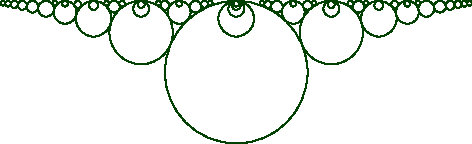
\includegraphics[width=9cm]{Cfarey_1.pdf}
 \caption{Cercles de Ford}
\end{figure}

\subsection*{Partie III.\quad Approximation de Dirichlet}
Soit $x$ irrationnel, il vient s'intercaler entre deux {\'e}l{\'e}ments cons{\'e}cutifs $\frac{p}{q}$ et $\frac{p^{\prime }}{q^{\prime }}$ de $\mathcal{F}_{Q}$. On dit que $\frac{p}{q}$ est la valeur approch{\'e}e par d{\'e}faut
de $x$ et $\frac{p^{\prime }}{q^{\prime }}$ celle par exc{\`e}s dans $\mathcal{F}_{Q}$. Consid{\'e}rons le m{\'e}dian $\frac{p+p^{\prime }}{q+q^{\prime }}$ et supposons par exemple
\[
\frac{p}{q}<x<\frac{p+p^{\prime }}{q+q^{\prime }}
\]
alors
\[
0<x-\frac{p}{q}<\frac{p+p^{\prime }}{q+q^{\prime }}-\frac{p}{q}=\frac{1}{q(q+q^{\prime })}
\]
Comme $\frac{p}{q}$ et $\frac{p^{\prime }}{q^{\prime }}$ sont cons{\'e}cutifs dans $\mathcal{F}_{Q}$ on a $q+q'>Q$ sinon le m{\'e}dian
viendrait s'intercaler. Ainsi
\[
0<x-\frac{p}{q}<\frac{1}{q(Q+1)}
\]
On peut donc choisir $a=p.$ On raisonne de la m{\^e}me mani{\`e}re lorsque $\frac{p+p^{\prime }}{q+q^{\prime }}<x<\frac{p^{\prime }}{q^{\prime }}$.\newline
Cette d{\'e}monstration est plus ancienne que celle de Dirichlet qui repose sur le principe des tiroirs.
\begin{quote}Lorsque strictement plus de $n$ objets sont rang{\'e}s dans $n$ tiroirs, l'un au moins des tiroirs contient plusieurs objets.
\end{quote}
